\documentclass{standalone}
\usepackage{tikz}
\usetikzlibrary{patterns, positioning}
\usepackage[sfdefault]{ClearSans} %% option 'sfdefault' activates Clear Sans as the default text font
\usepackage[T1]{fontenc}

\begin{document}
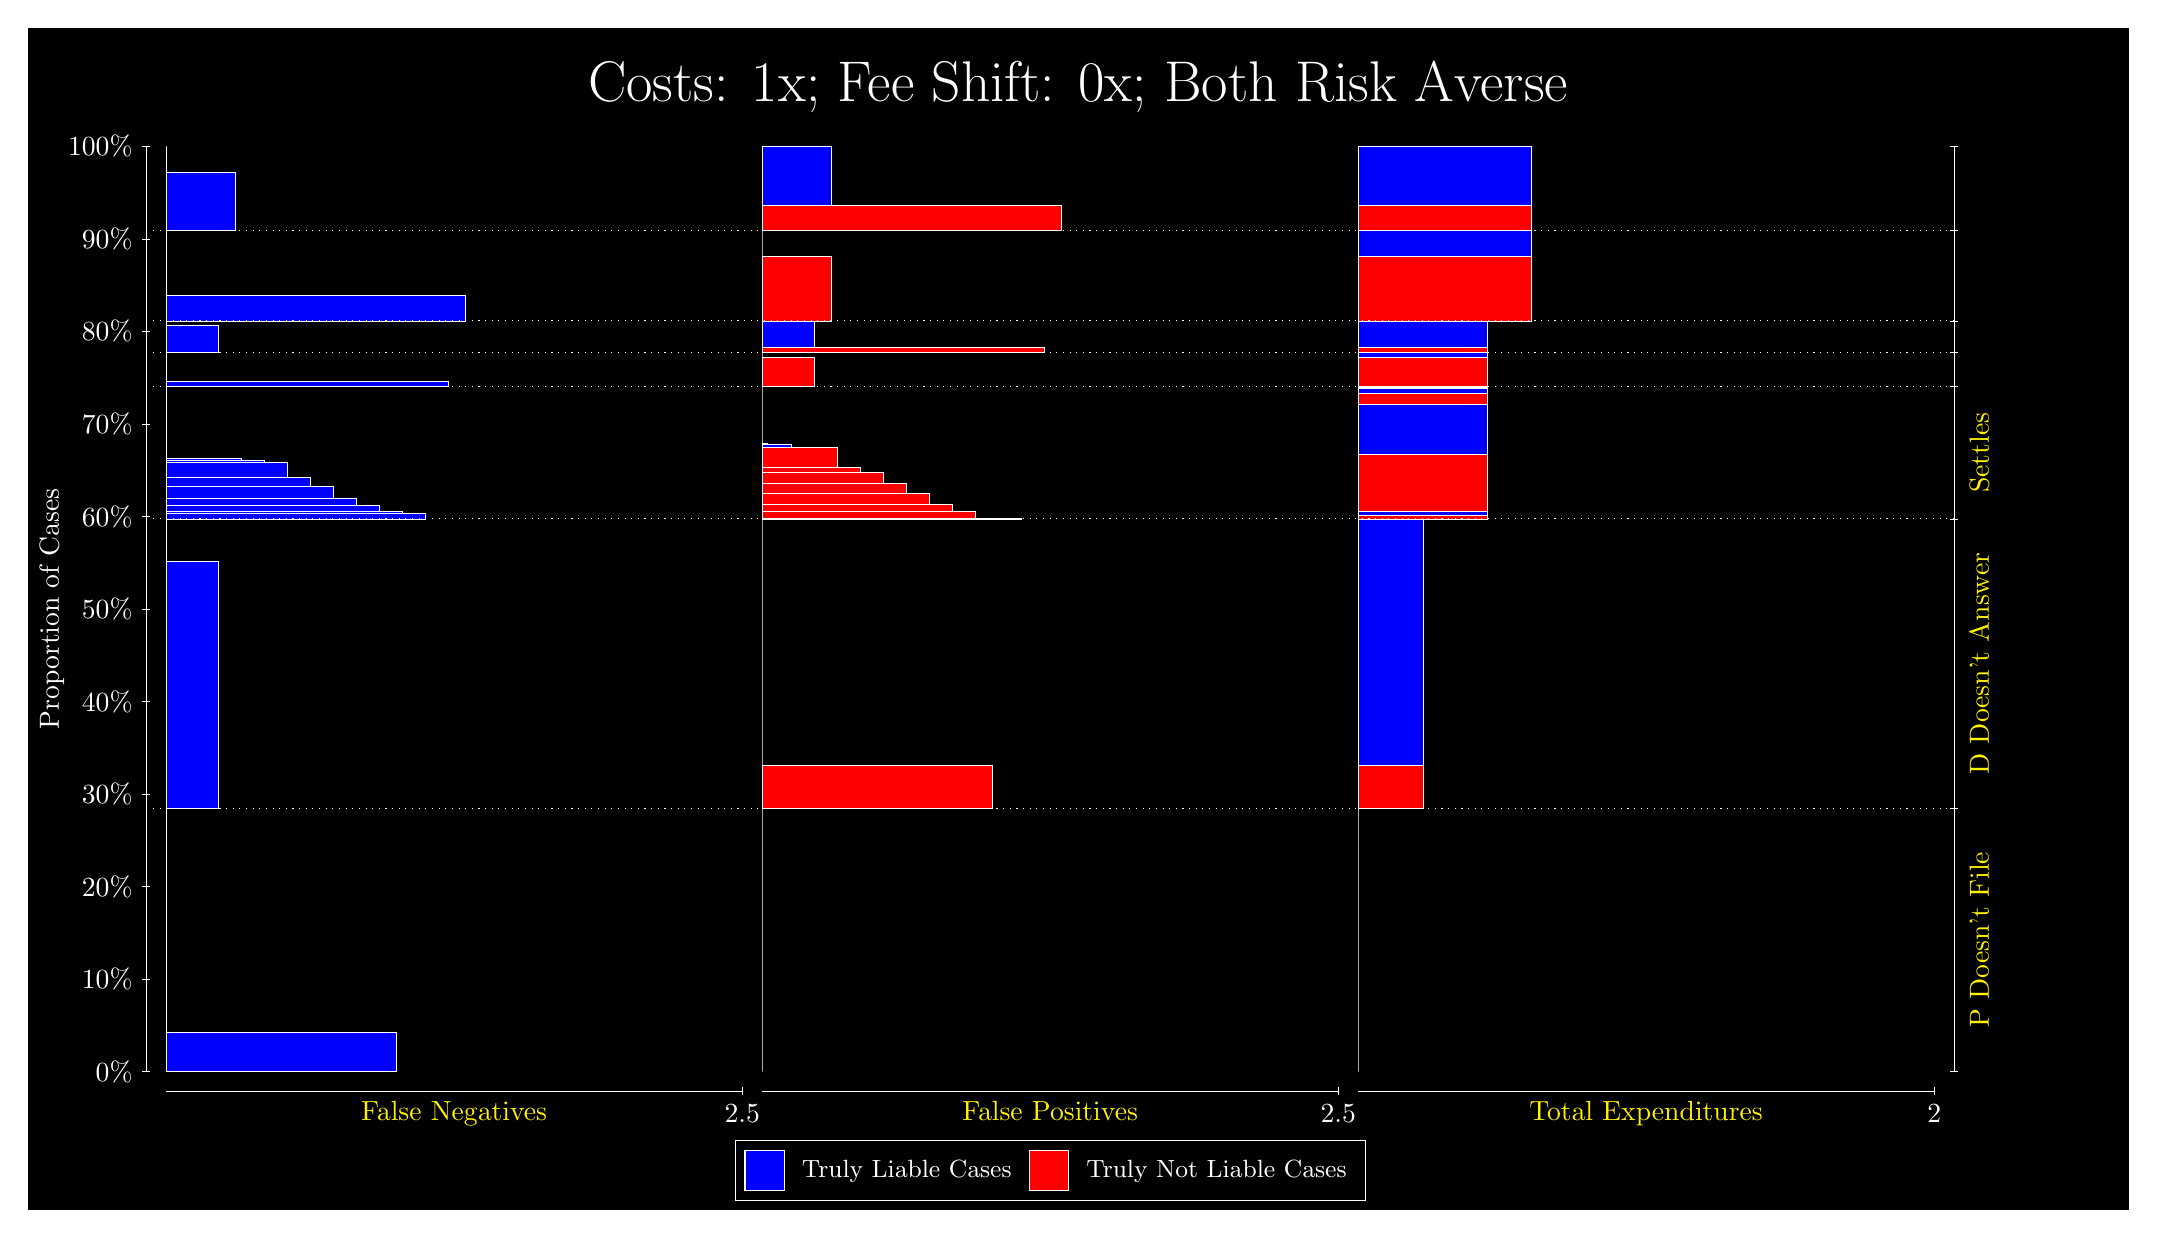
\begin{tikzpicture}
\draw[fill=black] (0,0) rectangle (26.667,15);
\draw[text=white] (0,13.5) rectangle (26.667,15) node[midway] {\huge Costs: 1x; Fee Shift: 0x; Both Risk Averse};
\draw[white, very thin] (1.5,1.75) -- (1.5,13.5);
\node[rotate=90, text=white, anchor=center] at (0.3, 7.625) {Proportion of Cases};
\draw[white, very thin] (1.45,1.75) -- (1.55,1.75);
\node[text=white, anchor=east] at (1.45, 1.75) {0\%};
\draw[white, very thin] (1.45,2.925) -- (1.55,2.925);
\node[text=white, anchor=east] at (1.45, 2.925) {10\%};
\draw[white, very thin] (1.45,4.1) -- (1.55,4.1);
\node[text=white, anchor=east] at (1.45, 4.1) {20\%};
\draw[white, very thin] (1.45,5.275) -- (1.55,5.275);
\node[text=white, anchor=east] at (1.45, 5.275) {30\%};
\draw[white, very thin] (1.45,6.45) -- (1.55,6.45);
\node[text=white, anchor=east] at (1.45, 6.45) {40\%};
\draw[white, very thin] (1.45,7.625) -- (1.55,7.625);
\node[text=white, anchor=east] at (1.45, 7.625) {50\%};
\draw[white, very thin] (1.45,8.8) -- (1.55,8.8);
\node[text=white, anchor=east] at (1.45, 8.8) {60\%};
\draw[white, very thin] (1.45,9.975) -- (1.55,9.975);
\node[text=white, anchor=east] at (1.45, 9.975) {70\%};
\draw[white, very thin] (1.45,11.15) -- (1.55,11.15);
\node[text=white, anchor=east] at (1.45, 11.15) {80\%};
\draw[white, very thin] (1.45,12.325) -- (1.55,12.325);
\node[text=white, anchor=east] at (1.45, 12.325) {90\%};
\draw[white, very thin] (1.45,13.5) -- (1.55,13.5);
\node[text=white, anchor=east] at (1.45, 13.5) {100\%};

\draw[white, very thin] (24.457,1.75) -- (24.457,13.5);
\draw[white, very thin] (24.407,1.75) -- (24.507,1.75);
\node[anchor=west] at (24.407, 1.75) {};
\draw[white, very thin] (24.407,5.0936) -- (24.507,5.0936);
\node[anchor=west] at (24.407, 5.0936) {};
\draw[white, very thin] (24.407,8.7686) -- (24.507,8.7686);
\node[anchor=west] at (24.407, 8.7686) {};
\draw[white, very thin] (24.407,10.451) -- (24.507,10.451);
\node[anchor=west] at (24.407, 10.451) {};
\draw[white, very thin] (24.407,10.886) -- (24.507,10.886);
\node[anchor=west] at (24.407, 10.886) {};
\draw[white, very thin] (24.407,11.284) -- (24.507,11.284);
\node[anchor=west] at (24.407, 11.284) {};
\draw[white, very thin] (24.407,12.431) -- (24.507,12.431);
\node[anchor=west] at (24.407, 12.431) {};
\draw[white, very thin] (24.407,13.5) -- (24.507,13.5);
\node[anchor=west] at (24.407, 13.5) {};

\draw[white, very thin, fill=blue] (1.75,1.75) rectangle (4.6775,2.2471);
\draw[white, very thin, fill=red] (1.75,2.2471) rectangle (1.75,5.0936);
\draw[white, very thin, fill=blue] (1.75,5.0936) rectangle (2.4087,8.2264);
\draw[white, very thin, fill=red] (1.75,8.2264) rectangle (1.75,8.7686);
\draw[white, very thin, fill=blue] (1.75,8.7686) rectangle (5.0435,8.8388);
\draw[white, very thin, fill=blue] (1.75,8.8388) rectangle (4.7507,8.8642);
\draw[white, very thin, fill=blue] (1.75,8.8642) rectangle (4.458,8.9359);
\draw[white, very thin, fill=blue] (1.75,8.9359) rectangle (4.1652,9.0325);
\draw[white, very thin, fill=blue] (1.75,9.0325) rectangle (3.8725,9.1807);
\draw[white, very thin, fill=blue] (1.75,9.1807) rectangle (3.5797,9.2937);
\draw[white, very thin, fill=blue] (1.75,9.2937) rectangle (3.287,9.4923);
\draw[white, very thin, fill=blue] (1.75,9.4923) rectangle (2.9942,9.5081);
\draw[white, very thin, fill=blue] (1.75,9.5081) rectangle (2.7015,9.5375);
\draw[white, very thin, fill=red] (1.75,9.5375) rectangle (1.75,10.451);
\draw[white, very thin, fill=blue] (1.75,10.451) rectangle (5.3362,10.519);
\draw[white, very thin, fill=red] (1.75,10.519) rectangle (1.75,10.886);
\draw[white, very thin, fill=blue] (1.75,10.886) rectangle (2.4087,11.225);
\draw[white, very thin, fill=red] (1.75,11.225) rectangle (1.75,11.284);
\draw[white, very thin, fill=blue] (1.75,11.284) rectangle (5.5558,11.609);
\draw[white, very thin, fill=red] (1.75,11.609) rectangle (1.75,12.431);
\draw[white, very thin, fill=blue] (1.75,12.431) rectangle (2.6283,13.175);
\draw[white, very thin, fill=red] (1.75,13.175) rectangle (1.75,13.5);
\draw[white, very thin, fill=red] (9.3189,1.75) rectangle (9.3189,4.5966);
\draw[white, very thin, fill=blue] (9.3189,4.5966) rectangle (9.3189,5.0936);
\draw[white, very thin, fill=red] (9.3189,5.0936) rectangle (12.246,5.6358);
\draw[white, very thin, fill=blue] (9.3189,5.6358) rectangle (9.3189,8.7686);
\draw[white, very thin, fill=red] (9.3189,8.7686) rectangle (12.612,8.7729);
\draw[white, very thin, fill=red] (9.3189,8.7729) rectangle (12.32,8.7769);
\draw[white, very thin, fill=red] (9.3189,8.7769) rectangle (12.027,8.8697);
\draw[white, very thin, fill=red] (9.3189,8.8697) rectangle (11.734,8.9479);
\draw[white, very thin, fill=red] (9.3189,8.9479) rectangle (11.441,9.0978);
\draw[white, very thin, fill=red] (9.3189,9.0978) rectangle (11.149,9.2241);
\draw[white, very thin, fill=red] (9.3189,9.2241) rectangle (10.856,9.3594);
\draw[white, very thin, fill=red] (9.3189,9.3594) rectangle (10.563,9.4184);
\draw[white, very thin, fill=red] (9.3189,9.4184) rectangle (10.27,9.682);
\draw[white, very thin, fill=blue] (9.3189,9.682) rectangle (9.6848,9.7115);
\draw[white, very thin, fill=blue] (9.3189,9.7115) rectangle (9.3921,9.7272);
\draw[white, very thin, fill=blue] (9.3189,9.7272) rectangle (9.3189,10.451);
\draw[white, very thin, fill=red] (9.3189,10.451) rectangle (9.9776,10.818);
\draw[white, very thin, fill=blue] (9.3189,10.818) rectangle (9.3189,10.886);
\draw[white, very thin, fill=red] (9.3189,10.886) rectangle (12.905,10.945);
\draw[white, very thin, fill=blue] (9.3189,10.945) rectangle (9.9776,11.284);
\draw[white, very thin, fill=red] (9.3189,11.284) rectangle (10.197,12.105);
\draw[white, very thin, fill=blue] (9.3189,12.105) rectangle (9.3189,12.431);
\draw[white, very thin, fill=red] (9.3189,12.431) rectangle (13.125,12.756);
\draw[white, very thin, fill=blue] (9.3189,12.756) rectangle (10.197,13.5);
\draw[white, very thin, fill=red] (16.888,1.75) rectangle (16.888,4.5966);
\draw[white, very thin, fill=blue] (16.888,4.5966) rectangle (16.888,5.0936);
\draw[white, very thin, fill=red] (16.888,5.0936) rectangle (17.711,5.6358);
\draw[white, very thin, fill=blue] (16.888,5.6358) rectangle (17.711,8.7686);
\draw[white, very thin, fill=red] (16.888,8.7686) rectangle (18.534,8.8181);
\draw[white, very thin, fill=blue] (16.888,8.8181) rectangle (18.534,8.8636);
\draw[white, very thin, fill=red] (16.888,8.8636) rectangle (18.534,9.5882);
\draw[white, very thin, fill=blue] (16.888,9.5882) rectangle (18.534,10.224);
\draw[white, very thin, fill=red] (16.888,10.224) rectangle (18.534,10.36);
\draw[white, very thin, fill=blue] (16.888,10.36) rectangle (18.534,10.431);
\draw[white, very thin, fill=red] (16.888,10.431) rectangle (18.534,10.435);
\draw[white, very thin, fill=blue] (16.888,10.435) rectangle (18.534,10.451);
\draw[white, very thin, fill=red] (16.888,10.451) rectangle (18.534,10.818);
\draw[white, very thin, fill=blue] (16.888,10.818) rectangle (18.534,10.886);
\draw[white, very thin, fill=red] (16.888,10.886) rectangle (18.534,10.945);
\draw[white, very thin, fill=blue] (16.888,10.945) rectangle (18.534,11.284);
\draw[white, very thin, fill=red] (16.888,11.284) rectangle (19.083,12.105);
\draw[white, very thin, fill=blue] (16.888,12.105) rectangle (19.083,12.431);
\draw[white, very thin, fill=red] (16.888,12.431) rectangle (19.083,12.756);
\draw[white, very thin, fill=blue] (16.888,12.756) rectangle (19.083,13.5);
\draw[white, dotted] (1.5,5.0936) -- (24.457,5.0936);
\draw[white, dotted] (1.5,8.7686) -- (24.457,8.7686);
\draw[white, dotted] (1.5,10.451) -- (24.457,10.451);
\draw[white, dotted] (1.5,10.886) -- (24.457,10.886);
\draw[white, dotted] (1.5,11.284) -- (24.457,11.284);
\draw[white, dotted] (1.5,12.431) -- (24.457,12.431);
\draw[white, very thin] (1.75,1.5) -- (9.0689,1.5);
\node[text=yellow, anchor=north] at (5.4094, 1.5) {False Negatives};
\draw[white, very thin] (9.0689,1.45) -- (9.0689,1.55);
\node[text=white, anchor=north] at (9.0689, 1.45) {2.5};

\draw[white, very thin] (9.3189,1.5) -- (16.638,1.5);
\node[text=yellow, anchor=north] at (12.978, 1.5) {False Positives};
\draw[white, very thin] (16.638,1.45) -- (16.638,1.55);
\node[text=white, anchor=north] at (16.638, 1.45) {2.5};

\draw[white, very thin] (16.888,1.5) -- (24.207,1.5);
\node[text=yellow, anchor=north] at (20.547, 1.5) {Total Expenditures};
\draw[white, very thin] (24.207,1.45) -- (24.207,1.55);
\node[text=white, anchor=north] at (24.207, 1.45) {2};

\node[text=yellow, centered, rotate=90] at (24.777, 3.4218) {P Doesn't File};
\node[text=yellow, centered, rotate=90] at (24.777, 6.9311) {D Doesn't Answer};
\node[text=yellow, centered, rotate=90] at (24.777, 9.6098) {Settles};





\draw (12.978300999999998,1.5) node[draw=none] (baseCoordinate) {};
\begin{scope}[align=center]
        \matrix[scale=0.5, draw=white, below=0.5cm of baseCoordinate, nodes={draw}, column sep=0.1cm]{
            \node[rectangle, draw, minimum width=0.5cm, minimum height=0.5cm, fill=blue] {}; &
            \node[draw=none, font=\small, text=white] (B) {Truly Liable Cases}; &
            \node[rectangle, draw, minimum width=0.5cm, minimum height=0.5cm, fill=red] {}; &
            \node[draw=none, font=\small, text=white] (B) {Truly Not Liable Cases}; \\
            };
\end{scope}

\end{tikzpicture}
\end{document}